\begin{figure}[h]
\centering
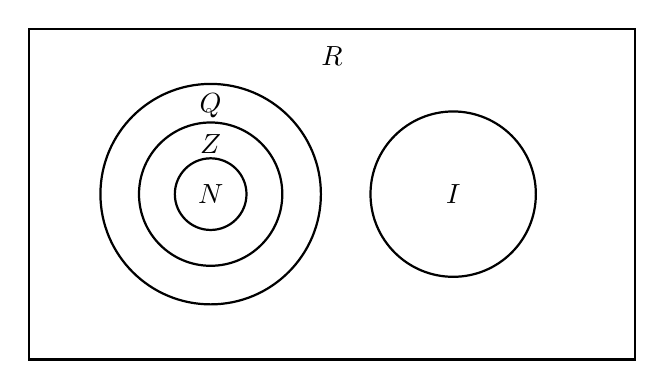
\begin{tikzpicture}[scale=0.7]
    % Real numbers rectangle (outermost)
    \draw[thick] (-5.5,-3) rectangle (5.5,3);
    \node at (0, 2.5) {$\mathbb{R}$};
    
    % Rational numbers circle (left side)
    \draw[thick] (-2.2,0) circle (2cm);
    \node at (-2.2, 1.6) {$\mathbb{Q}$};
    
    % Integers circle
    \draw[thick] (-2.2,0) circle (1.3cm);
    \node at (-2.2, 0.9) {$\mathbb{Z}$};
    
    % Natural numbers circle (innermost)
    \draw[thick] (-2.2,0) circle (0.65cm);
    \node at (-2.2, 0) {$\mathbb{N}$};
    
    % Irrational numbers circle (right side, disjoint)
    \draw[thick] (2.2,0) circle (1.5cm);
    \node at (2.2, 0) {$\mathbb{I}$};
    
\end{tikzpicture}
\captionsetup{width=0.8\textwidth}
\caption{\small{Hierarchy of number sets: Natural numbers ($\mathbb{N}$), Integers ($\mathbb{Z}$), Rationals ($\mathbb{Q}$), Irrationals ($\mathbb{I}$), and Real numbers ($\mathbb{R}$).}}
\label{fig:number_sets}
\end{figure}
